\chapter{Software Design}

This section will discuss the Software implementation of Verified
Boot. 
Verified Boot (Vboot) is a secure boot implementation only loads a
Kernel Image that has been signed by Google and is untampered.
Images that have been recognized as security risks will not be loaded and the system will restart into a Recovery Mode.
This section will discuss the security promises made by the system as well
as the attack vectors that are not considered.
It will also discuss relevant program flow and data structures.

\section{Security Promises}

The main purpose of Chrome OS's verified boot is to provide relative security to the end user without sacrificing usability or functionality. 
In its mission statement, verified boot is designed against an ``opportunistic hacker''~\cite{vboot-design-doc}.
Vboot protects against vectors of attack that are relatively quick to exploit.
Vboot will realize any attack or modification to the Image on the next boot cycle.
Once an attack is realized Vboot is responsible for forcing the system back into
a secure state.
For example, installing a malicious kernel driver to act as a keylogger would
alter the Image on the Chromebook.
The next time the Chromebook boots, Vboot will recognize that the Image changed,
and it will force the user to enter Recovery Mode and secure the device. 

There are many attacks that Vboot is not able to recognize or protect against.
For example, Vboot does not make any promises to the safety of the system once the kernel is running and the user has control. 
Any attacks that are outside of the Image (in userspace) would remain
undetected because they would not modify the kernel.
For example, changing the Web browser to use a proxy that collects information
would not be considered a kernel attack.
Userspace programs by definition have less access to the system and this reduces the severity and influence of the attack.
Possibly one of the biggest flaws is that any attack to the kernel during
runtime would remain until the system was powered down.
In certain situations this could provide plenty of time for an attack to steal valuable data.
However, such an attack is outside the scope of this paper.

\section{Verified Boot Flow}

In order to make Vboot modular and extensible for future platforms, Google has split the process into three main sections as seen in Figure~\ref{fig:vboot_stages_overview}.
This split allows Google to make the Read-Only stage as small as possible, which
is desirable because bugs in this stage cannot be fixed.
These sections are referred to as Read-Only (RO) Firmware, Read-Write
(RW) Firmware, and Kernel.
These sections are run in sequence with each section attesting the section that comes later.
The Root of Trust begins in the Read-Only section.
This section is assumed to be unmodified because it is read-only.
Then each section attests that that next section is signed by Google and
unmodified. 
In this way, the Root of Trust builds until all of the system's code is
attested, and the laptop can boot.

For the scope of this document only the attestation the Read-Only Firmware's
attestation of the Image will be discussed.
The Read-Only attestation contains more interesting control flow, and
attestation process is essentially repeated for the Read-Write Firmware.

\begin{figure}
\begin{subfigure}{.4\textwidth}
  \centering
  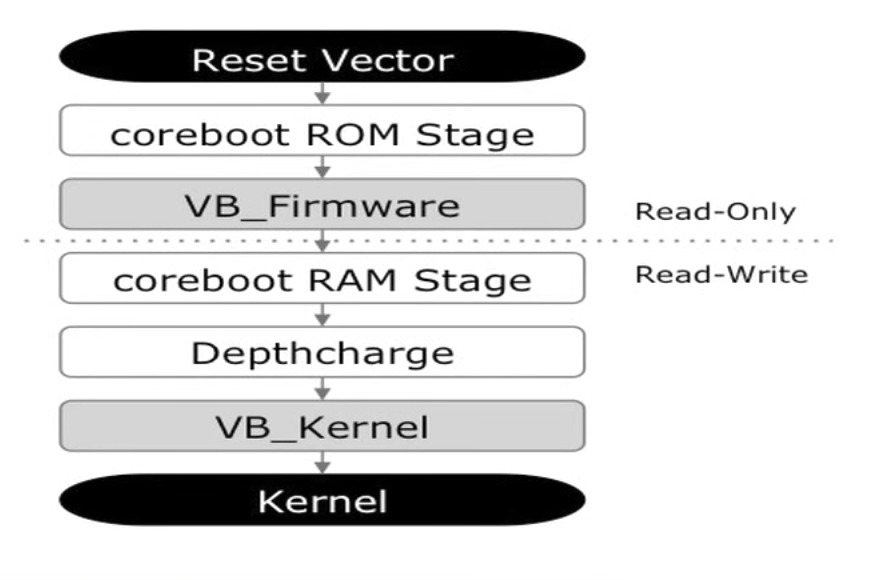
\includegraphics[width=1.0\linewidth]{vboot_stages_overview.png}
\end{subfigure}
\begin{subfigure}{.60\textwidth}
  \centering
  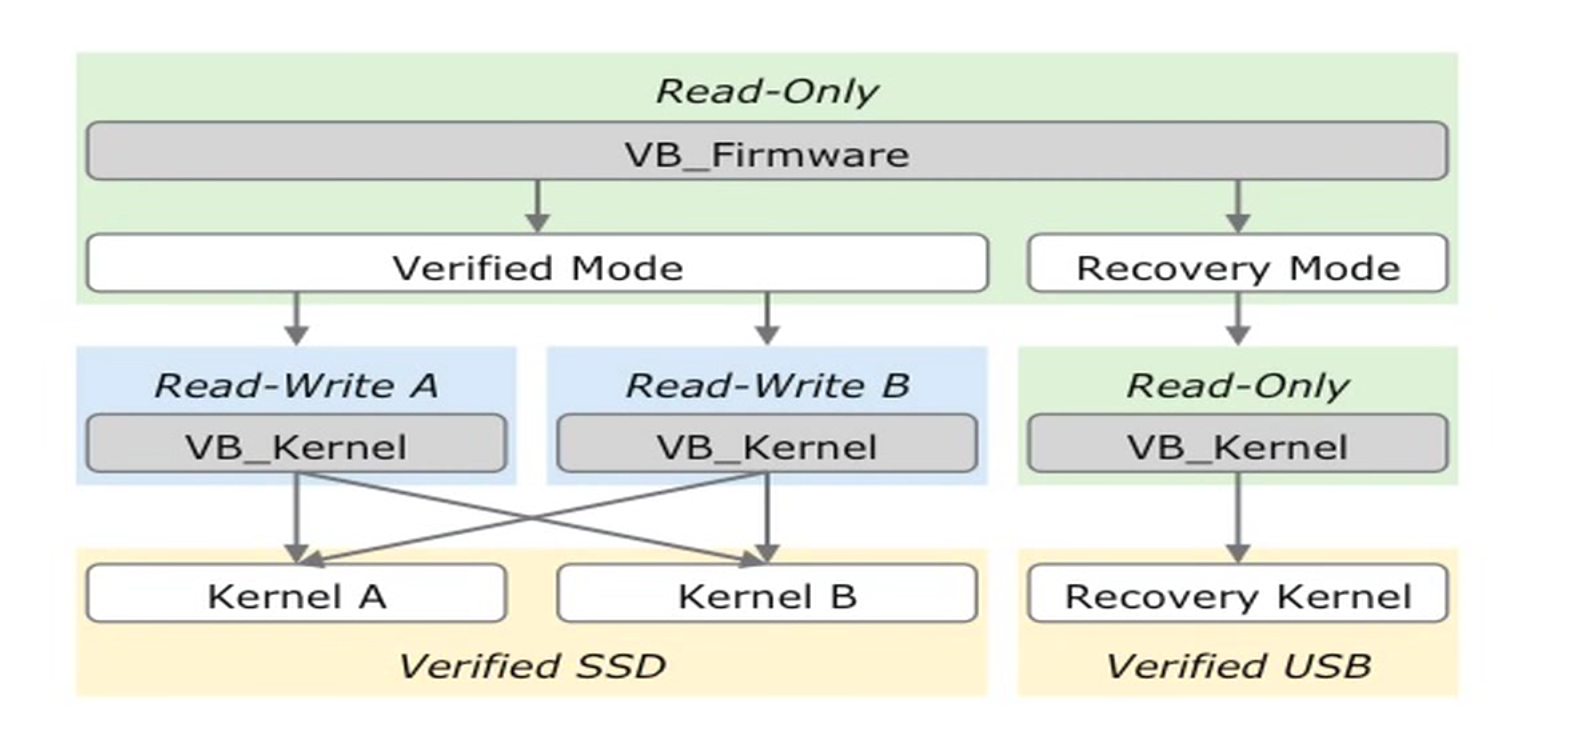
\includegraphics[width=1.0\linewidth]{vboot_stages_AB_recovery.png}
\end{subfigure}
\caption[Verified Boot Stages]{The left image shows the stages of Vboot Firmware. The right image
shows the different boot paths, and data locations. Both make the distinction
between Read-Only and Read-Write memory.}
\label{fig:vboot_stages_overview}
\end{figure}

The Read-Only Firmware of Vboot is responsible for attesting Google's Image. 
Vboot contains all of the code and hardware drivers it needs to accomplish this task.
It verifies the Image signature using Google's main public key.
This public key is also read only so it is guaranteed to be secure.
The Read-Only Firmware is also responsible for the transitions between Developer Mode, Safe Mode, and Recovery Mode.
These transitions will be described in more detail in Section~\ref{sec:boot-modes}.

\begin{figure}
  \centering
  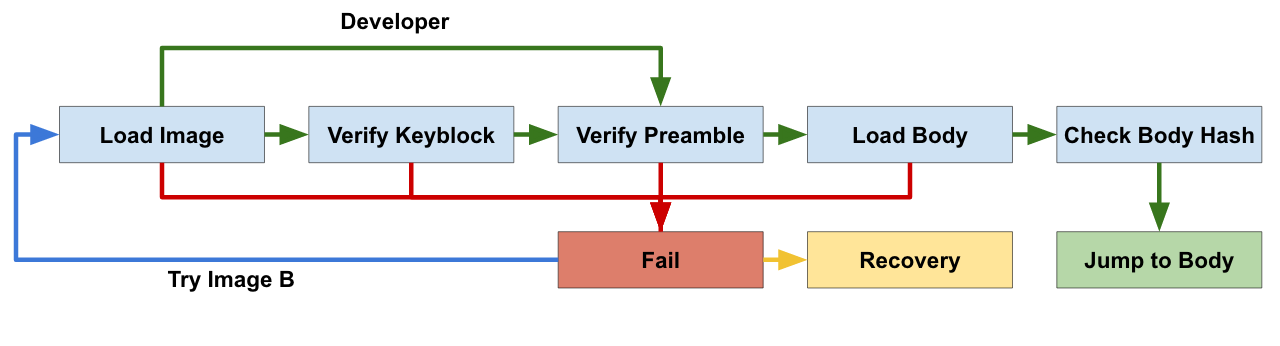
\includegraphics[width=0.8\linewidth]{verification_flow.png}
  \caption[Verified Boot Program Flow]{The logical flow for attesting the Image. Notice
  the different path for Developer mode, and the possibilities for
  failure.}\label{fig:verif_flow}
\end{figure}
\begin{figure}
  \centering
  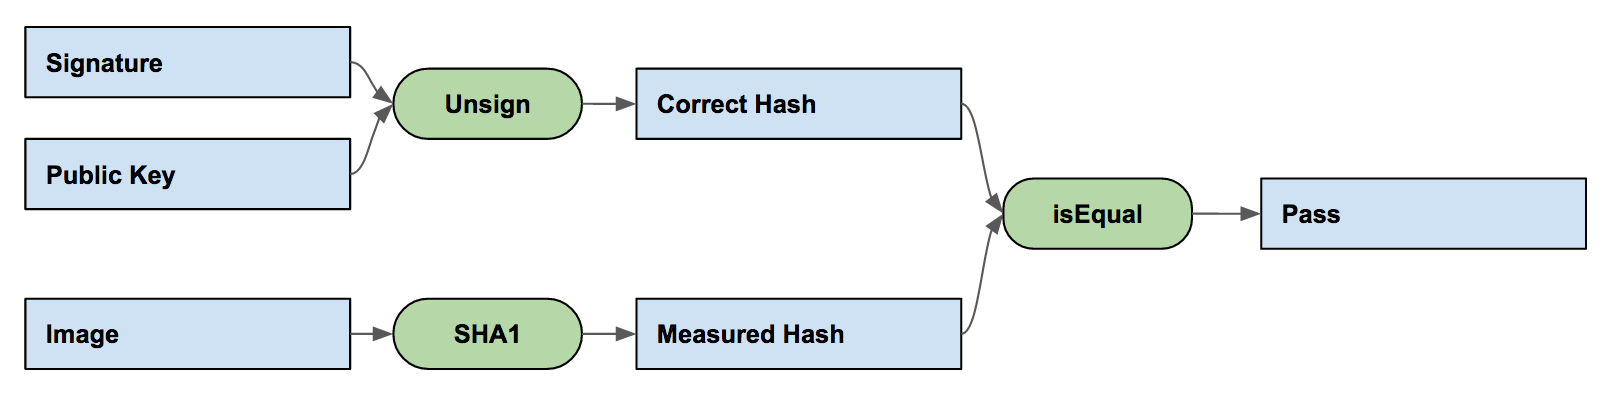
\includegraphics[width=0.8\linewidth]{attest_flow.png}
  \caption[General Attest Flow]{The logical flow for attesting any data
      structure.}\label{fig:attest_flow}
\end{figure}

Vboot's process for attesting the Image is described as follows: Vboot first
loads the image, then attests the keyblock, then attests the
preamble, then attests the body, and finally Vboot executes the code in the body. 
These stages can be seen in Figure~\ref{fig:verif_flow}.

Loading the image consists of copying the image out of the Flash Memory and into
RAM\@.

Verifying the Keyblock consists of using the Keyblock's signature, which is a
hash of the Keyblock that is signed by Google's Private key.
Google's Public Key is used to decrypted the signature.
Once decrypted the signature is is now a hash of the Keyblock.
Finally, Vboot hashes the Keyblock, and this value is compared with the
decrypted signature.
If the hashes are not equal, then Vboot can be sure that the Keyblock has been
modified in some way. 

The Preamble is attested in the same way, except that a different Private and Public Key pair is used.
The Keyblock holds the key that is used for the Preamble's signature.
The Keyblock is used so that Google has the ability to change the encryption
type of the Preamble and Firmware if they wish.
Google's Main Public Key is stored in Read-Only memory, so it cannot be changed.
This hierarchy of keys also allows Google to be less careful with their ``lower
security'' keys because they can change them through a firmware update if the key is
compromised.

After the Preamble is verified, the Image is hashed and compared
against the hash stored in the preamble. 
The hash in the preamble has already been attested because the preamble was
signed, so this attests that the Image is correct and unmodified. Finally, the
system jumps to the Image and begins to execute the code for the 
Operating System.


\section{Boot Modes}\label{sec:boot-modes}

Vboot has three major boot modes that influence the program's behavior.
The first is the Secure mode which goes through the full process of Verified Boot.
The second mode is the Recovery mode which allows for a broken machine to
format all memory and transition to Secure Mode.
The third mode is the Developer mode and in this mode the RSA signature is not verified.
The Developer mode exists so that hobbyists can write their own firmware boot code and run operating systems other than Chrome OS\@.

The transitions allowed between the modes can be seen in
Figure~\ref{fig:mode_fsm}.
On each transition, Vboot is responsible for taking steps to ensure that
security is preserved. 
These responsibilities are also seen in the figure.

\begin{figure}
  \centering
  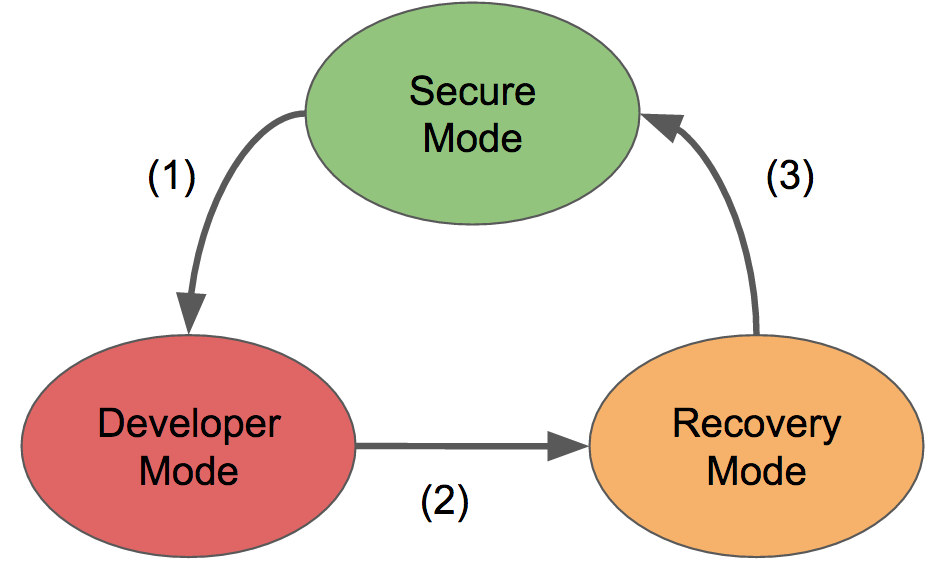
\includegraphics[width=0.4\linewidth]{mode_fsm.png}
  \caption[Vboot Boot Mode FSM]{The FSM for the boot modes. \\
  1. The TPM's nonvolatile storage and keys are wiped. The user's data
  is erased. \\
  2. The laptop is booted into Recovery, Vboot installs a Chrome USB.
  \\
  3. The TPM's storage goes through reconfiguration. The entire disk is wiped.
  \\}\label{fig:mode_fsm}
\end{figure}

\subsection{Developer Mode}

Developer mode poses interesting security questions to Verified boot because it
disables Vboot's security guarantees that the OS has been signed by Google~\cite{developer-mode}. 
To allow the existence of Developer mode, but still maintain 
Secure Mode, there are various requirements around the Developer mode transition.
First, a physical presence is required to fully complete the Developer mode transition. 
This means that a user must press a certain key combination (Control + D) when
the developer mode screen appears at boot time.
The physical presence exists such that developer mode cannot be enabled through an off-site software attack without the user's knowledge.
The developer mode screen is referred to internally as the ``Scary Screen'', and its purpose is also to prevent users from being tricked into enabling developer mode by an external phishing party.

In order to prevent an attacker from enabling Developer Mode so that they could
read or write to secure storage, Vboot wipes all secure storage on the transition into Developer Mode.
The secure storage that is wiped includes the RSA keys and various secrets stored in the TPM and the partion on disk where user data is stored.
Wiping this data on the transition is necessary for the confidentiality of the system and failure to do so is a security risk.

These precautions are also taken on the transition from Developer Mode to Safe Mode. 
If secure storage is left untouched moving from Developer Mode to Safe Mode, then an attacker would be able to place potentially malicious information in secure storage.
Vboot assumes that the secure storage can only be written to and read from by
Google, and this assumption is violated in Developer Mode. 
Wiping all secure storage on this transition is the easiest way to ensure that the platform has full control.
The precautions mean that on the transition from Developer to Safe Mode, the system has to go through Recovery Mode.

\subsection{Recovery Mode}

Recovery Mode is responsible for getting the system back to a secure state.
Recovery Mode will be activated automatically when an error is recognized by Vboot.
This error could range from hardware failures to a corrupted image to a detected attack on the system.
When the system boots into Recovery it requests a Recovery Image stored on external memory, either an SD card or a USB drive.
Recovery Mode uses Google's Recovery RSA keypair.
Google's Recovery public key is stored in Read-Only Memory for security.
Recovery Mode does full attestation of the Recovery Image, and if the Image
passes then it will overwrite the Images stored in main memory.

Recovery mode is responsible for wiping secure memory, mainly the user's disk partition and TPM's secure storage.
If Recovery completes successfully, the system is in a secure state and Vboot can then continue safely.
Recovery is also the only mode that disables Vboot's rollback detection.
Often if there are problems with an Image update, Recovery mode is the only way
to install an older Image. 

\section{Data Structures}\label{sec:data-structures}

To start understanding the Vboot process of attesting the Image, it is necessary
to talk about the Image's data structures.

\subsection{Google's Image}

\begin{figure}
    \centering
    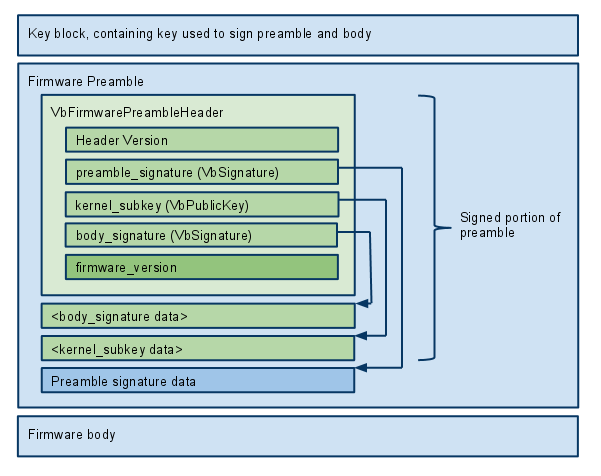
\includegraphics[width=0.6\linewidth]{fw_image.png}
    \caption[Google's Image Data Layout]{Layout of Google's Image~\cite{vboot-data-structures}}
    \label{fig:vboot_images}
\end{figure}

The actual Image is not a data structure but a chunk of data that is loaded
contiguously into RAM\@.
The image structure, as seen in Figure~\ref{fig:vboot_images}, consists of three
parts: the Key Block, the Preamble, and the main body of the image.
The Key Block is attested first using Google's public key stored in Read Only memory.
Once the Key Block has been shown to be safe, the Key Block's public key will be used to verify the preamble.
The Preamble contains a hash of the Image's body.
The Image's body contains the code that is going to be run next.
Vboot attests the body by hashing it and comparing that value against the hash
stored in the Preamble.

\subsection{Key Blocks}\label{sec:key_block}

\begin{figure}
\begin{subfigure}{.5\textwidth}
  \centering
  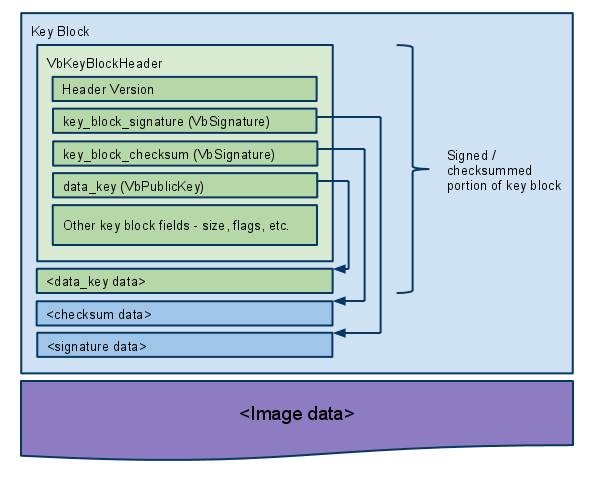
\includegraphics[width=1.0\linewidth]{vboot_keyblock.png}
\end{subfigure}
\begin{subfigure}{.20\textwidth}
  \centering
  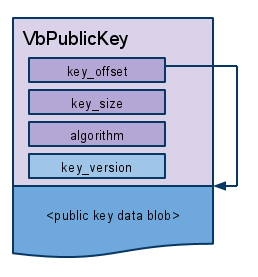
\includegraphics[width=1.0\linewidth]{vbpublickey.png}
\end{subfigure}
\begin{subfigure}{.20\textwidth}
  \centering
  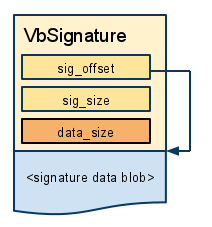
\includegraphics[width=1.0\linewidth]{vbsignature.png}
\end{subfigure}
\caption[Key Block Data Structure]{The Key Block data structure and the data
structure for Keys and Signatures}
\label{fig:vboot_keyblock}
\end{figure}

The Key Block is the data structure that allows a hierarchy of RSA keys to be used during Vboot.
Figure~\ref{fig:vboot_keyblock} shows the structure of the Key Block. 
The Key Block flags are used to determine which mode of Vboot the Keyblock is valid in. 
There are 4 possible boot modes corresponding to the combination of the two binary options, Developer and Recovery.
% info located in vboot_struct.h

Within the Key Block there exists data structures for a public key and a signature.
Google has added the ability to change their encryption strength.
They have added support for RSA 1024, 2048, 4096, 8192 and for SHA 1, 256, 512, for a total of 12 different possible algorithm combinations.

\subsection{Google Binary Block}

% info found in gbb_header.h
The Google Binary Block (GBB) is a part of Vboot's Root of Trust.
It is a data structure stored in Read-Only memory that is initialized and configured in the factory at the laptop's creation.
It contains the Root and Recovery RSA keys, a host of flags that affect boot
operation, and the bitmaps used for the Vboot screen displays.


\section{Code Organization}

Like most modern operating systems, Chrome OS is written in C.
Like Linux, Chrome OS is maintained using Git for version control. 
Git is a diff-based, non-centralized version control system that makes it easy for programmers to share code, rollback changes, and maintain separate branches of the same codebase~\cite{git}.
Google has built a tool called ``repo'' that is used on top of git~\cite{repo}. 
Repo is a tool to manipulate multiple code repositories. 
It's primary benefit is that it allows a company to specify how multiple git repositories should be installed and placed within a given file-system.
This is both helpful and necessary as Chrome OS consists of over one thousand different external and internal repositories. 

Coreboot, vboot\_reference, and depthcharge, are the repositories used by Google
for Verified Boot.
The flow of Verified Boot through the repos can be seen in
Figure~\ref{fig:code_repos} and the purpose of each repo is described below.

\begin{figure}
  \centering
  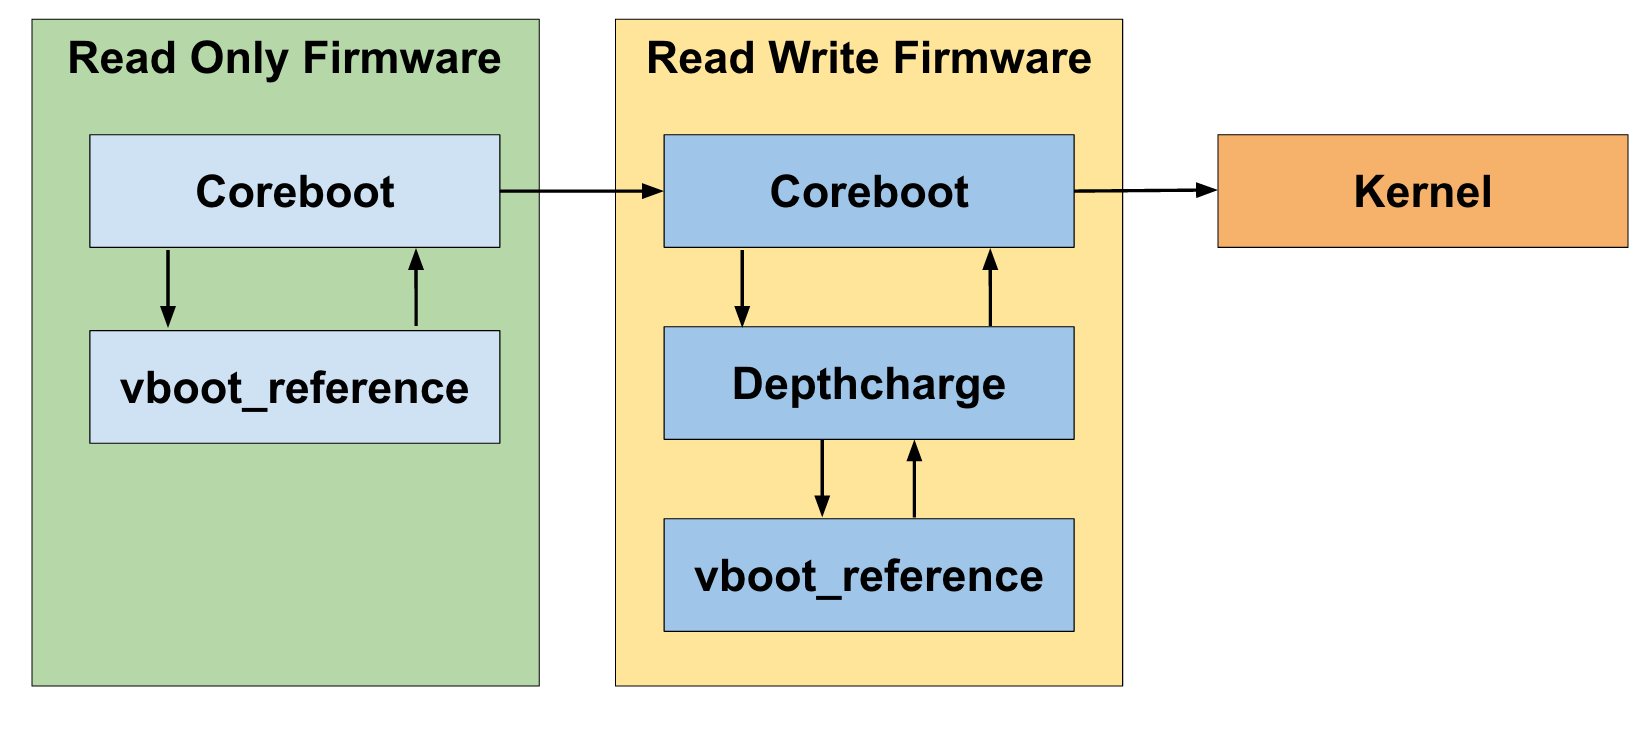
\includegraphics[width=0.8\linewidth]{code_repos}
  \caption[Vboot Repository layout]{ChromeOS's boot flow goes through Coreboot, Depthcharge, and the Vboot Library twice for Firmware and Kernel verification}\label{fig:code_repos}
\end{figure}

\begin{figure}
  \centering
  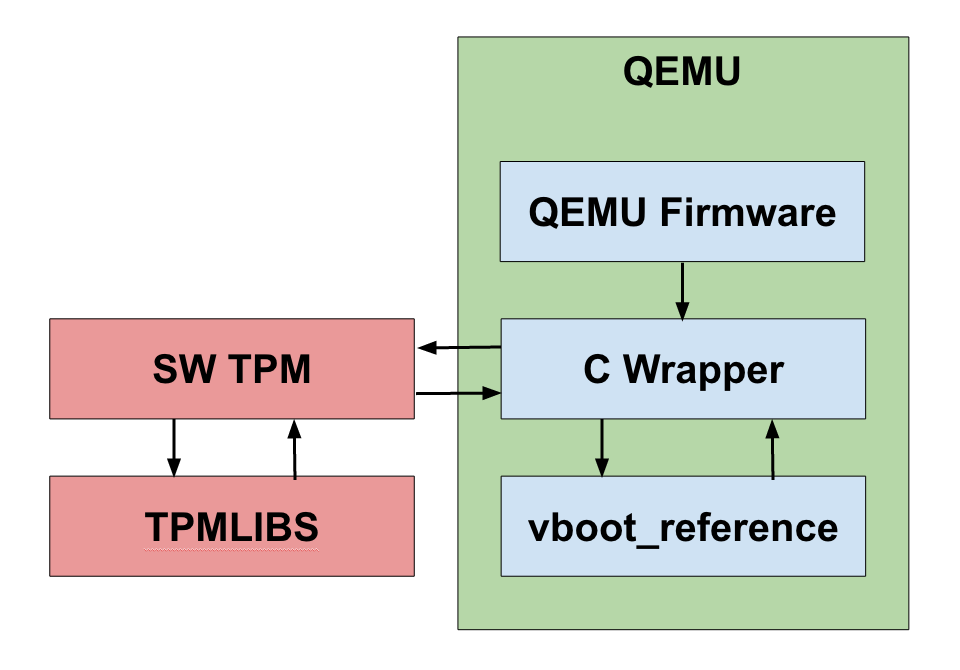
\includegraphics[width=0.45\linewidth]{qemu_repos}
  \caption[This report's Repository Layout]{This report's boot flow uses a
      created C wrapper for interfacing with QEMU and the TPM, and an unmodified Vboot for the verification}\label{fig:qemu_repos}
\end{figure}

\subsection{Coreboot and Depthcharge}\label{coreboot}

Coreboot is a fully Open-Sourced alternative to traditional BIOS implementations.~\cite{coreboot}
It is lightweight and is configured to implement the full standard of the Unified Extensible Firmware Interface (UEFI).
Google has chosen Coreboot because of its small code footprint, full extensibility, and the fact that it is available freely as an Open Source project.

The Coreboot code is responsible for doing very early initialization code on the main CPU\@. 
% This includes things like setting up the GPIO pins, enabling hardware interrupts, setting up a large stack in RAM, and providing driver callbacks to the payload that it will eventually call.
Coreboot is setup so that once a baseline level of initialization is complete, it passes control to another section of code called a ``payload''~\cite{coreboot-payload}.
This payload is responsible for initializing the more specialized drivers, and the concept of a payload means that Google can keep support more hardware without altering the Coreboot source code.

The payload that Coreboot calls to further initialize the Chromebook is Depthcharge.
Depthcharge contains platform specific functions like reading and writing
commands to the TPM, or interacting with the SHA accelerator. 
The vboot\_reference library will make calls back into Coreboot for platform
specific access. 
As this report was run on an emulated Chromebook and not a real platform, the
Coreboot + Depthcharge repositories were replaced by new code in the CMBC-Vboot
repo.

\subsection{Vboot\_reference}

The vboot\_reference repo contains all of the control and algorithms for the vboot process~\cite{vboot-codebase}.
The repo is designed such that it does not rely on any knowledge about the platform.
If a function requires usage of a driver or something that is board specific, it will make a callback into Depthcharge which will provide the relevant information.
Again, for this report, Depthcharge will be replaced by the CBMC-Vboot
repository.

One of the more helpful features of the vboot\_reference repo is that it can be
built in a stand-alone fashion as a C archive file.
More information about building the project can be found in the appendix, but
this feature allowed the Vboot functions to be placed into the QEMU environment
easily and be adapted for many different types of hardware.

\subsection{Software TPM}

The Software TPM was taken from a series of repositories created by IBM's
Stefan Berger. 
These repositories emulated the TPM functions\cite{TPMLibs}, the TPM Command
Fifo\cite{SWTPM}, and the TPM Register Interface\cite{TPMQEMU}. 
appendix.

This emulated TPM implements all of the TPM's functionality as defined by the
TCG Standards.
Software emulation was desirable over a physical chip for many reasons.
First, for security reasons, the state of a hardware TPM is difficult to modify.
If testing required forcing the TPM into a particular state, it may involve
manual power restarts and multiple calls to the TPM library.
The Software TPM allows state to be saved, restored, and modified on the fly
without going through the TPM API.
Second, a Hardware TPM's operations would be a black box.
The Software TPM's code is open source and can be inspected manually.

When the Software TPM is passed to QEMU, it is accessed through the 
Registers outlined in Section~\ref{sec:TPM}.
This is the same way that the Vboot TPM library accesses the TPM, so these
functions can be used unmodified. 

\subsection{CBMC-Vboot}

The CBMC-Vboot is a repository created to connect Vboot to the emulated
hardware used in this report\cite{my-repo}.
The layout of this repository is discussed in the Appendix.
We can see in Figure~\ref{fig:qemu_repos} that it is used as a wrapper to tie
Vboot together with QEMU and the Software TPM libraries.
